\chapter{Introduction}
\label{ch:introduction}

%I like what Hall-Lew (2009) has done with her first chapter. Project overview, sociophonetics in general, summary of regional, state, and city English studies, and then (because she focuses on ethnicity) an overview of ethnicity.

Compared to many other regional varieties of English in the United States, there is far less research on Western American English. This may be due to a variety of factors, such as being settled later than other regions and its generally low population density. In particular, it may be because English in the region has relatively few language features that are stigmatized nationwide. One of the participants for this study, whom I will call Shane, expressed this sentiment in an interview:
\begin{num_quote}
    I'm more of a, ``Hey, you sound like you're from Boston,'' ``Hey, you sound like you're from New York,'' y'know? Whereas I've never heard anybody say, ``You sound like you're from Seattle,'' y'know. So, I mean we \textit{must}. I mean, we \textit{must} have a different dialect. But how it would compare to others\ldots? (Shane, M, b. 1971)
\end{num_quote}
There are people in the West, and they do use language. What do westerners sound like and how does their speech compare to other North American varieties of English?

In this study, I describe the speech of 54 residents of Cowlitz County in southwestern Washington State. Using traditional data collection techniques and innovative statistical modeling, I show that Shane was right: they \textit{do} have a different dialect. And I will also answer his trailing question and show how their speech compares to other varieties of English in the West.

This dissertation is a direct response to the calls for action put forth by the editors in the \textit{Speech in the Western States}. The last sentences in the first two volumes are, respectively:
\begin{quote}
    Regardless of what we uncover as we move forward, it is clear that speech in the West is dynamic and changing, and there will be plenty to keep dialectologists busy in the coming years. \citep[164]{fridland_etal_2016_pads}.
\end{quote}
\begin{quote}
    So, now the vowels of the West are perhaps not so wild as we once thought, but there is much left along the Western frontier for future generations of dialectologists to explore. \citep[173]{fridland_etal_2017_pads}.
\end{quote}
It is my hope that this work expands our knowledge of speech in this region and furthers our understanding of language change in North American English.


% TODO Renwick: tone of this section is a bit informal & self-dismissive?
\section{Why Cowlitz County?}
\label{sec:why_cowlitz_county}

I first became acquainted with Cowlitz County while I was engaged to my wife, since it is where she grew up. While I did not notice any particular speech patterns (at that time I did not know that I would be studying dialectology), I did notice that the people were particularly friendly and chatty. In January 2015, we took advantage of the Linguistic Society's annual meeting in Portland to visit family again. I did not present anything at that conference, but I attended many of the presentations of the American Dialect Society, way up on the 23rd floor. One of those sessions was on speech in the West. I was not aware at the time, but those presentations were among the first on English along the Pacific coast, particularly in the Pacific Northwest, and some of them later became part of the first volume of \textit{Speech in the Western States} \citep{fridland_etal_2016_pads}. After listening to those presentations, my main takeaway was that there were interesting phenomena occurring in the West but that there is still much more research to be done in the Pacific Northwest.

There are several reasons why Cowlitz County was selected as the field site for this study. First, to be clear, my parents-in-law have lived in Kelso since 1995, and even though they are not natives to the area, they are integrated culturally and socially into the community. For a researcher to study their family’s community is not uncommon in sociolinguistics. \citet{hazen_2000_pads} mentions that he, too, studied his in-laws and their community. \citeauthor{hall_lew_2009_diss}'s \citeyearpar{hall_lew_2009_diss} research on the Sunset District in San Francisco was facilitated by her grandmother living there for over 30 years, and this shared connection allowed for more comfortable and lengthier interviews. And \citeauthor{bowie_2000_diss}'s \citeyearpar[41]{bowie_2000_diss} research in Waldorf, Maryland included his immediate family and friends. It is far easier to find participants in a community when a researcher has an “in” than it is to do a cold call and hope to find participants in that way.

But having family and personal contacts in the area were not the only reasons Cowlitz County is the topic of this dissertation. (After all, I had family in half a dozen other relatively small towns in various other states.)
It is true that an in-depth analysis of speakers from this region dutifully fills this gap in the dialectological map of North American English, but there are many other communities in the United States that have had relatively little research\footnote{In fact, if filling in a geographic gap were my sole objective, a cheaper and easier alternative would have been to study speech in Athens, Georgia!}. What does an analysis of Cowlitz County offer besides documenting yet another speech community?

Cowlitz County, Washington was chosen as the field site for this study because of the historical connection between the timber industry and the city of Longview. As explained in detail in chapter \ref{ch:cowlitz_county}, Longview was founded in 1923 in conjunction with the establishment of the Long-Bell company. I initially hypothesized that the speech of the mill workers would be different in some way from other residents in the community. So far, I have not yet found evidence to support this hypothesis, but I have found that the changing industry practices in the 1970s did trigger the loss of traditional linguistic features and the spread of innovative patterns into the county \citep{stanley_2018_pwpl}. Regardless of the role the milling companies play on the area, for a relatively small and isolated community to experience a massive cultural and demographic shift as newcomers immigrated to work at the mills is likely to have ramifications on the speech in the area. For this reason Cowlitz County is an ideal site in the study of dialect mixture and its effects on speech in the area after nearly a century of change.

The speech of Cowlitz County residents also provides additional insight into how the concept of Place plays a role in sociolinguistic variation. Linguists have often noted how the importance of particular locale to an individual can be reflected in their speech \citep{labov_1963, johnstone_etal_2002, carmichael_2014_diss, reed_2018}. As explained in \S\ref{sec:then_and_now}, some residents of Cowlitz County have strong feelings towards Longview and its history. For example, the Longview '23 Club honors the original settlers of the city. Those who are proud of their local heritage stand in contrast to relative newcomers to the city and this contrast manifests itself linguistically.

Finally, Cowlitz County's relative size and population density combined with its position between Portland and Seattle makes it an ideal place for how sociolinguistic variables diffuse geographically. While the speech of Portland and Seattle are similar, there are measureable differences \citep{becker_etal_2016_pads, wassink_2016_pads}. The relatively rural Cowlitz County offers a unique insight into language outside of major metropolitan areas. Identifying how Cowlitz County fits into Pacific Northwest English can help understand language change.



\section{English in Cowlitz County}

Even among Washingtonians, the speech of Cowlitz County does not stand out. In a study of the perception of Washington English, \citet{evans_2011} finds that, in a draw-a-map task, many people circled other parts of the state and gave them labels such as ``country'', ``Spanish'', ``slang'', or ``pronuncation'', but Cowlitz County was rarely included in these circled areas.

Though there is still much work to be done, linguists know considerably more about Western American English(es) than we did even fifteen years ago. While the number of studies focused on westerners has increased steadily over the past couple decades, there has been an explosion of research just in the past five years. Some areas have received more attention and researchers have shifted from simple documentation to more nuanced, theoretical topics. In other areas, like Montana, New Mexico, Wyoming, and Idaho, the number of sociophonetic studies---collectively---can still be counted on one hand.

To my knowledge, no part of southwest Washington, including Cowlitz County, has been the focus of any linguistic research. Speakers from this region have been included in some regional and national-level surveys of North American English, but no more than a few speakers have been sampled.




\subsection{Early work}

While studies in pronunciation have always been a part of sociolinguistic research, many of the early publications in American dialectology were compiled word lists of lexical items particular to some community. From its beginning, one goal of the American Dialect Society was to document ``strange, uncommon, or antiquated words or uses of words really current in any community'' \citep[18]{sheldon_1889}. The scope and size of these early wordlists varied considerably, ranging from case studies on particular words or phrases \citep{pound_1929, pearce_1958} to the \textit{Dictionary of Regionalisms} \citep{bartlett_1848}.

Many of these early word lists were published in \textit{Dialect Notes}, the American Dialect Society's first series, or its successor, \textit{American Speech}. Of the western states, one finds the most on communities in California, such as terms originating from the gold rush \citep{hamilton_1932, moore_1926}, from California old fields \citep{pond_1932}, peculiarities used by California poets \citep{grant_1942}, words from the \textit{Dictionary of Regional English} that seem to have originated in California \citep{shulman_1949}, and general California-isms \citep{lehman_1921, watkins_mulhall_1951}. Other regions had general word lists as well, such as Colorado \citep{davidson_koehler_1932}, Oregon \citep{hausen_1931}, Wyoming \citep{clough_1936, clough_1954}, and Washington \citep{adams_1958}, but they are less frequent. Within these states, there were a few articles on the words used by specific groups of people, such as gold and silver miners \citep{davidson_1929}, whitewater rafters \citep{akin_goltry_1969}, fire fighters \citep{yelsma_1969} in Colorado, as well as religious groups in Idaho and Wyoming \citep{jensen_1931, lindsay_1933}. As for the Pacific Northwest, some articles provide general wordlists \citep{harvey_1914_part1, harvey_1914_part2, finder_1965} or of industry-specific terms from the region like from workers at shipyards \citep{babbitt_1944}, truck drivers \citep{hanley_1961}, and painters \citep{hines_1969}. Because of the prevalence of some industries in the Pacific Northwest, there are numerous reports of wordlists associated with loggers \citep{stevens_1925, davis_1942, davis_1950, carranco_1956, mcculloch_1958} and railroad workers \citep{batie_1934, schultz_1937, snapp_logan_1938, cottrell_montgomery_1943} and, in one case, both \citep{carranco_1962}. This collection of early reports on lexical items illustrates that there were some researchers thinking about language in the West, though relatively few compared to other regions.

To my knowledge, the earliest phonetic description of English in the Pacific Northwest Washington is \citet{stevens_1925}. In addition to the many words and expressions used by loggers, a description of pronunciation itself can be found towards the end of the article---a rare find for publications at that time:
\begin{quote}
    ``Attempting to describe the loggers' speech in a phrase, I would say that it is a chesty one, like that of the old time sailors. A logger must shout at his work, and he naturally picks words that will roar out of his chest. Words with short \textit{u} and \textit{e}, broad \textit{a}, and long \textit{o} sounds. Perhaps this is why he uses `holy' and `old' so much when he swears. The ring in his speech is unlike the twang one hears on the drawl of the cowboys'' \citep[139]{stevens_1925}.
\end{quote}
The description of these vowels and voice quality is subjective and lacks detail (i.e., what are the phonetic correlates to ``chesty''?). However, another brief description of the consonants provides perhaps a small amount of additional detail:
\begin{quote}
    ``The logger smothers such consonants as \textit{m} and \textit{s}, and he drops the first \textit{h} as carelessly as a Cockney, for he will breathe a whole sentence out of his chest in one exhalation, cutting his words and fitting the loose ends together. Often he refuses the long \textit{i}. `I'm going home` he turns into something like `mm go nome.' `I can' always interests me as the logger pronounces it. ``Ahkn' resembles the sound he makes, but I can no more than give a hint here of the chesty \textit{n} sounds he throws into `I can,' `he can,' and the like'' \citep[139]{stevens_1925}.
\end{quote}
Unfortunately, these vague descriptions of Pacific Northwest English are the only of their kind. And they only describe (presumably) men who work as loggers and do not generalize to other people living in the Pacific Northwest. Furthermore, their subjective nature does not allow for easy comparison to contemporary data. Thus for the first half of the twentieth century, while other areas were being described in great detail, the Pacific Northwest was an enigma to dialectologists.

\subsection{The Linguistic Atlas of the Pacific Northwest}

It took until the 1950s for more rigorous phonetic descriptions of speakers in this area to be published. The \textit{Linguistic Atlas of the Pacific Northwest}, directed by Carroll Reed and David Carlson, with Henry Person and David DeCamp assisting in the fieldwork, was the first project that analyzed the pronunciation of speakers in the Pacific Northwest (that is, Washington, Oregon, and Idaho) with enough detail to allow for some comparison to modern techniques. In some regions, the Linguistic Atlas projects were published as a complete set of bound volumes, like the \textit{Linguistic Atlas of New England} \citep{kurath_1939_lane} and the \textit{Linguistic Atlas of the Upper Midwest} \citep{allen_1973_laum}. Unfortunately, the \textit{Linguistic Atlas of the Pacific Northwest} was one of the many that did not\footnote{The phonetic transcriptions of the targetted words from these interviews are now housed at the University of Kentucky. I do not know whether these interviews were recorded, but if they were, those recordings have been lost.}, so the findings are not available in an accessible way\footnote{\citet[186]{allen_1977} states that progress was hindered in part because Reed moved from the University of Washington eventually to the University of Massachusetts. Reed stated in personal communication with Allen that he would like to resume fieldwork after retirement, though I do not know if that ever happened.}.

The only results from that project are found in brief, scattered reports by Caroll Reed \citeyearpar{reed_1952, reed_1956, reed_1957, reed_1961, reed_1967}. In them, we learn that the low back vowels are close or merged, in many people's speech, particularly in western Washington and in children, though with a number of lexical exceptions \citeyearpar[Reed][]{reed_1952}. We also find variation in linguistic features such as the \textit{Mary-merry-marry} merger, the retention of /\textipa{\*w}/, /\textipa{\*r}/-intrusion in words like \textit{wash}, back vowel mergers before laterals, and lexical variation like the vowel quality in \textit{root}, \textit{roof}, and \textit{greasy}. There is also some evidence that sound changes that have been later documented to exist in the region, such as /o/-fronting and \beg-raising, were in their beginning stages. However, there is also no evidence of other features that contemporary Pacific Northwesterners exhibit, such as the raising of /\textipa{\ae}/ before nasals or before /\textipa{g}/. These early reports illustrate that the Pacific Northwest was comprised of people coming from a variety of speech backgrounds and that at least by the 1950s, a single, unified variety had not yet emerged.

Because of the large amount of variation, Reed was optimistic that linguistic research in the Pacific Northwest would provide fruitful area for future dialectologists:
\begin{quote}
    "[T]he present study may provide a beginning for the eventual much more intensive study which is soon to be made in this region. With all the laboratory tools at his command---settlement history, family history, and every kind of dialect mixture and linguistic diversity---the linguist may find here, to say the least, an ideal ground for experimental research" \citeyearpar[Reed][189]{reed_1952}.
\end{quote}
However, Reed never saw this eventual intensive study come forth. To my knowledge, there was very little additional research on the region for several decades. It took until the 20th Century for focused research on the region to resume. In Chapter \ref{ch:lit_review}, I provide a more in-depth of these contemporary studies since they more directly relate the the current study.

Before continuing, it is important to discuss whether these early works are representative of English in Cowlitz County. The closest speaker from the \textit{Linguistic Atlas of the Pacific Northwest} was a woman from Oakville, Washington, some 60 miles to the northwest of Cowlitz County. Under the assumption that the Pacific Northwest is a relatively homogeneous dialect area, perhaps Reed's early reports are representative. However, this is an assumption that remains to be tested empirically.

\subsection{Large-scale projects}

Focused research on the Pacific Northwest (and especially Cowlitz County) was sparser than it was on other dialect areas. However, in the past century, various researchers have carried out several nation-wide studies and have included participants from the Pacific Northwest. Is Cowlitz County represented in these large-scale projects, and if so, what do these projects tell us about English in the region?

One of the earliest unified, nation-wide projects that documented speech English in the United States was what \citet[216--217]{allen_1977} calls the \textit{Thomas Collection}. As early as the 1930s and especially after World War II, Charles Thomas took advantage of new recording technology and sent blank tapes to colleagues across the country with instructions to find local speakers to read specific passages. He collected recordings from 15,000 individuals, representing 2,500 of the 3,000 counties. This study culminated in his \citeyear{thomas_1958} book \textit{An Introduction to the Phonetics of American English}. In many cases, his findings coincided with what fieldworkers for the Linguistic Atlas Projects described, but for other things they did not. In fact, \citet{foster_hoffman_1966} noticed some discrepancies with what Thomas described for Pacific Northwest English and published a ``correction'' for speakers in the Seattle area.

Another early regional study was the \textit{Dictionary of Regional American English} \citep{cassidy_2013_dare}, which sought to document lexical regionalisms in the mid 20th Century. To my knowledge, the fieldwork associated with that project was the first linguistic project to include a speaker from Cowlitz county, speaker WA030 from Castle Rock. A full analysis of this one speaker in relation to the rest of the Washingtonians is out of the scope of this study, but that project does offer one small glimpse into how speakers from Cowlitz County spoke decades ago.

Finally, some Cowlitz County residents were sampled in a collection of more than 700 questionnaires that were mailed to Washington, Oregon, and Idaho \citep[61,103--116]{reed_1967}.\footnote{According to Map 20 (Reed \citeyear[104]{reed_1967}), it appears that eight individuals were sampled from Cowlitz County.} That data shows that some people used the terms \textit{darning needle} for `dragonfly', \textit{quarter to} and \textit{quarter of}, \textit{barnyard} for `corral', \textit{grate} for `andirons', \textit{Dutch cheese} and \textit{smearcase} for `cottage cheese', and \textit{steps} or \textit{stoop} for `back porch'. However, because of the nature of mail-in responses, pronunciation was not analyzed in these samples.

More contemporary dialect studies have included speakers close to Cowlitz County. For example, the \textit{International Dialects of English Archive}\footnote{\scriptsize https://www.dialectsarchive.com} includes ones speaker from Vancouver, Washington, which is one county south of Cowlitz County. The \textit{Atlas of North American English} \citep{labov_ash_boberg_2006_anae} had some speakers from Washington (Seattle, Spokane, Walla Walla) and Oregon (Portland, Eugene, and Oregon City), but none came from areas near Cowlitz County. Other online-based studies such as the \textit{Harvard Dialect Survey} \citep{vaux_golder_2003} and Josh Katz' New York Times--based dialect survey \citep{katz_2016} did not collect acoustic data, and because the data for those projects are unavailable, it is unknown whether Cowlitz County speakers are represented.

In summary, it appears that while areas near Cowlitz County have been sampled in various regional and national dialectology projects, very little data has been collected from Cowlitz County itself. There are likely other pockets of the United States that have been similarly overlooked, but one purpose of this study is to fill in that gap in our dialectological map of the United States in order to get a more complete picture of speech in the Pacific Northwest.


\section{Variables of study}

When documenting the language of a community for the first time, the researcher is presented with numerous aspects of language that need to be described, including variation in phonetic, morphological, syntactic, and lexical structures. A dissertation can only be so large, so it is then up to the researcher to decide which variables deserve the most attention.

The questionnaires used in the \textit{Linguistic Atlas of the Pacific Northwest} covered many linguistic features, and Reed's work has illustrated a large amount of variation in these phonetic structures. While preparing to conduct fieldwork for this project (described in \S\ref{fieldwork}), I sought to target linguistic features that were variable in those early works. Some of these included vowels before laterals and rhotics, and the raising of front vowels before /\textipa{g}/, and in \citet{stanley_2017_ADS, stanley_2018_pwpl} I provide an analysis of these features.

Nevertheless, after the fieldwork was completed, it had come to my attention that a different set linguistic variables may be a more salient source of variation in this community, especially in the context of how it appears to have diffused across the West. The lowering and retraction of front lax vowels /\textipa{I, E, \ae}/, which I am calling the \textit{Elsewhere Shift}\footnote{See \S\ref{sec:terminology} for an explanation of why this name was chosen over the (many) others in circulation.}, the raising of /\textipa{\ae}/ before nasals, and the low back merger are highly variable across the western states and have been shown to index many different social meanings. This study contributes to this growing knowledge of the Elsewhere Shift by analyzing the vowels' formant trajectories and their variation and social meaning in a timber-based Washington community. Figure \ref{fig:elsewhere_shift_diagram} illustrates the Elsewhere Shift in the vowel space. The general counterclockwise motion of these shifts follows the general principals of language change that are known to occur in other varieties of English and in other languages \citep{labov_1994, harrington_etal_2011}.

\begin{figure*}[tb!]
    \centering
    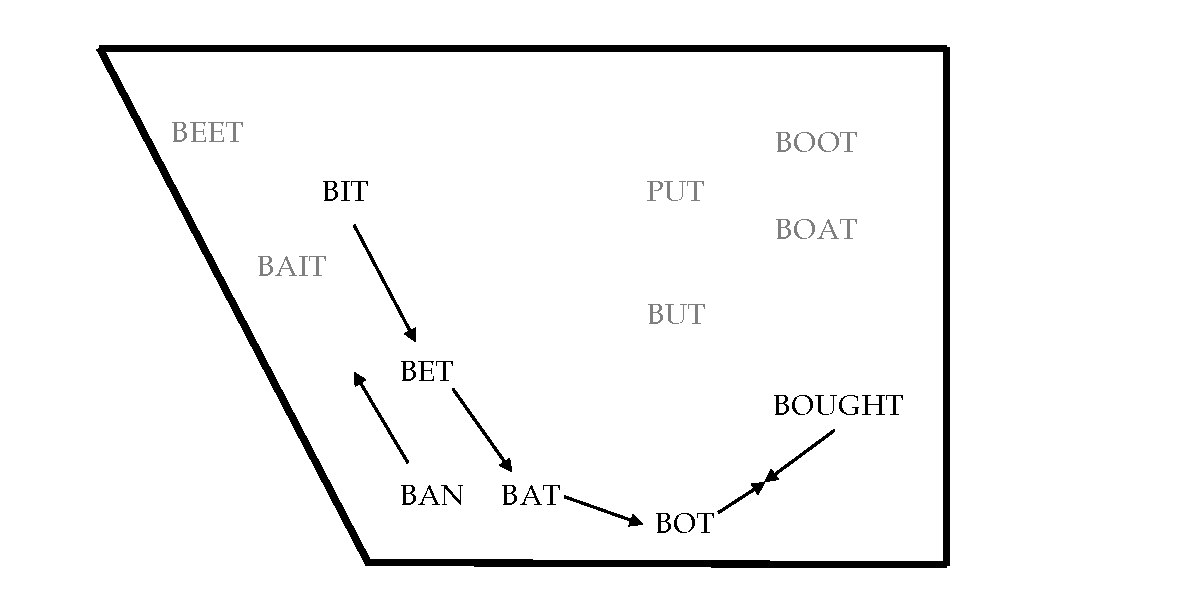
\includegraphics[width = 6.5in]{Figures/other_figures/cvs_diagram.pdf}
    \caption[The Elsewhere Shift]{The Elsewhere Shift. Vowels not included in this study are grayed out. Back vowel fronting, which some consider to a part of the Elsewhere Shift, is not indicated on this diagram.}
    \label{fig:elsewhere_shift_diagram}
\end{figure*}

Before proceeding, it is important to establish the labeling conventions that will be used for the remainder of this study. Of the labels that already exist to refer to vowels, such as IPA (/\textipa{\ae}/, /\textipa{E}/, /\textipa{I}/) and the set used by Labov and Trager \& Bloch (/\textipa{\ae}/, /\textipa{E}/, /\textipa{i}/), I have chosen to use the Wells lexical sets (Wells 1982: xviii–xix) when referring to broad phonetic categories\footnote{See also \citealt[43]{kennedy_grama_2012}, \citealt{fruehwald_2018}, and \citealt{stanley_2019_blog} for explanations of label conventions.}, which are written in {\sc small caps} (i.e. \trap, \dress, \kit). However, when referring to allophones of these vowels, I use a mix of labels, some conventional and others less so. For example, recent volumes in the \textit{Publication of the American Dialect Society} series follow \citet{eckert_2008} and Thomas \& Yaeger-Dror's \citeyearpar{thomas_yaegerdror_2009} example of using the frame {\sc b\_t} (i.e. \bat, \bet, \bit) instead of the Wells labels. I likewise follow this convention, but only in reference to the elsewhere allophone of the phoneme itself. This makes it clear that, for example, \kit refers to the phoneme /\textipa{I}/ and \bit refers to any realization of \kit that is before obstruents. I likewise use the frame {\sc b\_n} for prenasal allophones (\ban, \ben, \bin). A more complete description of each of the allophones and their labels can be found in \S\ref{corpus_size_constitution}.




\section{The current study and organization of chapters}

This study documents the Elsewhere Shift in speakers from Cowlitz County, Washington. In addition to describing language in understudied and recently settled region of the country, this study utilizes a different method in the study of vowels that has not been fully explored in American English dialects. Specifically, I use generalized additive mixed-effects models to analyze the formant dynamics of these vowels. While some researchers have analyzed vowel trajectory in relation to the Elsewhere Shift in the West, this study is the first to use this particular statistical model. Not only does this technique provide additional clarity in the realization of these vowels, but it uncovers variation in a vowel's \textit{trajectory}---not just relative \textit{position}---that has not been reported in other western communities.

In Chapter 2, I provide a more thorough review of the literature in relation to speech in the West and the Elsewhere Shift. This shift is not yet fully understood, and different communities undergo the shift in different ways. I pay particular attention to the regional distribution of the Elsewhere Shift, pointing out that it has not yet been described in Washington. I also illustrate the conflicting accounts of how the shift is progressing in these different regions. I describe the structural relationship between the vowels, and theoretical accounts for the shift (i.e., whether it is a pull chain, a push chain, or a parallel shift). I also devote attention to the social meaning of the Elsewhere Shift, and what speakers index and listeners perceive when innovative variants are used.

Before moving to the study, I pause and use chapter 3 to outline the history of Cowlitz County. There were three reasons for the inclusion of this chapter. First, because this is the first linguistic analysis in this community, I felt it was appropriate to provide additional context so that the reader may better understand the geography, history, and culture. Second, Washington was settled relatively late compared to the rest of the country and Cowlitz County especially was even later than other parts of the Pacific Northwest. In fact, we have a record of the names and origins of the first white settlers were the area now known as Cowlitz County; the Founder Effect \citep{mufwene_1996} may be an important factor when explaining language in this area. Finally, I include this chapter because in the results chapters, I find that major historical events (the founding of Long-Bell in the early 1920s, and the change in the timber industry in the late 1970s) correlate with linguistic changes in the area.

Chapter 4 describes the methods used in this study. Sociophonetic research involves many steps to get from fieldwork to statistical analysis. I explain the traditional fieldwork methodology utilized in this study, transcription, forced alignment, formant extraction, filtering, and normalization procedures. For some of these data processing tasks, I describe a few methods that are reported in the literature, evaluate the pros and cons of each method, and justify why I selected the procedure used here. I then describe the corpus size and constitution, providing a full description of the vowel classes in this study. Because sociolinguistic research is becoming increasingly quantitative in nature, I then provide a brief history of the methods used in variationist studies, justify the need for analyzing vowel dynamics, and describe how generalized additive mixed-effects models were implemented. Finally, I describe how vowel shifting has been quantified in other studies and why I believe the typical method (comparing formant values to the ``benchmarks'' in the \textit{Atlas of North American English}) is inappropriate. It is my hope that this chapter provides a useful summary of the methods used in variationist studies and that others may become more informed regarding the statistical and analytical tools they use.

Chapters 5--7 present the results of this study. Chapter 5 deals with the front lax vowels before obstruents and demonstrates that the Elsewhere Shift is very much present in Cowlitz County speakers. Chapter 6 focuses on these three vowels before nasals, establishing that the prenasal split applies only to \trap and not \dress or \kit. I also focus on these vowels before /\textipa{N}/ because they appear to exhibit a different type of variation than the other prenasal environments, and because a full account of these vowels, particularly their formant trajectories, has not been completed in the West. Finally, Chapter 7 presents results from the low back vowels, illustrating that the two vowels are not fully merged, but that they have been in a state of near-merger for several generations. At the end of each of these chapters, I discuss what the implications are for these findings, such as how the vowels are structurally related, what the results say about the diffusion of the shift, and a justification for the use of generalized additive mixed-effects models.

In Chapter 8, I summarize the findings and focus on a different source of data---the \textit{content} of the interviews---to describe the social meaning of the Elsewhere Shift. While a full-fledged 3rd Wave \citet{eckert_2012} analysis was not employed in this study, these speaker comments do illustrate a small portion of what these shifted vowels mean. Furthermore, I show that while older people enjoy their community, younger people do not and instead orient themselves towards Portland.\footnote{It is noteworthy that the younder speakers' orientation is towards the nearest urban center rather than an urban center within their own state. It is common in dialectology research to focus on a single US state. A fruitful area of research would focus on state boundaries and how dialect features and speaker orientation crosses those boundaries, such as the Kansas-Missouri state line \citet{strelluf_2019} and the United States--Canada line \citet{swan_2016_diss}.} This drastic generational shift can be explained by considering the history of the community, particularly the economic recession in the 1970s and 1980s, and I suggest here that these major historical events were perhaps the reason for the adoption of innovative speech variants by the youngest generations.


Finally, in Chapter 9, I provide an overview of the work, discuss the limitations and point out directions for future work. In particular, I list many of the infrequent linguistic variables that were heard among these speakers, suggesting a high degree of variation in this community.

In addition to these chapters, I have also included several appendices. Some include supplementary methodological information like the reading passages, wordlist, and minimal pairs used in the interview and the list of stopwords that were excluded from analysis. Other appendices are related to the statistical output because they are too large to be comfortably included in the results chapters: summaries of the statistical models, model comparisons, and large multi-panel plots that show difference smooths and spectrogram-like visualizations. References to specific tables and visualizations are included throughout the text and this PDF includes internal hyperlinks to help guide the reader to this supplementary material.

It is my hope that this work succeeds in filling in one small hole in our dialect map of the United States and that the thorough description of vowel dynamics here will serve as a useful point of comparison in future studies on vowel trajectories.
